\documentclass[a4paper, 10pt, final, garamond]{book}
\usepackage{cours-preambule}

\raggedbottom

\makeatletter
\renewcommand{\@chapapp}{Induction -- chapitre}
% \renewcommand\thechapter{1 et 2}
\makeatother

\begin{document}
\setcounter{chapter}{2}

\chapter{Correction du TD}
\section{Étude qualitative de l'induction}
\label{sec:indqualicorr}

\begin{enumerate}
	\item Dans toutes ces situations, on a un aimant proche d'un solénoïde non
	      alimenté, formant un circuit fermé par un ampèremètre. Selon
	      l'orientation de l'aimant, il y a initialement dans le solénoïde un
	      champ magnétique dirigé vers la gauche ou la droite (les lignes de champ
	      sortent par le Nord et rentrent par le Sud), et le déplacement de
	      l'aimant va venir faire varier son amplitude dans un sens ou l'autre.
	      \bigbreak
	      Or, par la loi de \textsc{Faraday}, on sait qu'une variation de flux
	      dans un circuit électrique est à l'origine d'une tension induite en son
	      sein, et donc à une intensité induite si le circuit est fermé. On sait
	      de plus qu'une spire de courant parcourue par une intensité électrique
	      est à l'origine d'un champ magnétique $\vv{B}$ dirigé
	      perpendiculairement au plan de la spire et dont le sens respecte la
	      règle de la main droite (version tire-bouchon).
	      \bigbreak
	      De plus, avec la loi de modération de \textsc{Lenz}, on sait que les
	      effets de l'induction modèrent les causes qui lui ont donné naissance.
	      Ainsi, la \textbf{variation du flux extérieur} dû au mouvement de
	      l'aimant sera \textbf{modéré par la création du champ induit}.
	      \bigbreak
	      On va donc déterminer physiquement le sens de $\vv{B_{\rm ind}}$ dans le
	      solénoïde pour répondre à la loi de \textsc{Lenz}, et vérifier s'il
	      correspond au sens du champ $\vv{B}$ qu'on aura en prenant $I > 0$ sur
	      les différents graphiques. Il serait aussi possible de raisonner à
	      partir de la première situation uniquement, et en répercutant ensuite
	      les relations entre les causes sur les relations entre les conséquences.
	      \begin{enumerate}
		      \item Le champ magnétique initial dans le solénoïde est dirigé vers
		            la gauche. En déplaçant l'aimant vers la gauche, son amplitude à
		            l'intérieur du solénoïde augmente également dans ce sens. Le
		            champ induit est donc \textbf{vers la droite} pour compenser
		            cette augmentation vers la gauche. L'intensité représentée doit
		            donc être \textbf{négative}.
		      \item Le champ magnétique initial est dirigé vers la gauche. En
		            déplaçant l'aimant vers la droite, son amplitude décroît donc
		            vers la gauche (ou augmente vers la droite)~: le champ induit
		            est donc \textbf{vers la gauche}. Ceci s'obtient bien avec
		            $\mathbb(I>0)$ avec la règle de la main droite.
		            \bigbreak
		            On peut aussi remarquer qu'on ne fait que changer le sens de
		            déplacement de l'aimant par rapport à la première situation, et
		            qu'on s'attend donc en effet à trouver une conséquence opposée.
		      \item Le champ magnétique initial est dirigé vers la droite. En
		            déplaçant l'aimant vers la gauche, son amplitude augmente vers
		            la droite~: le champ induit est donc \textbf{vers la gauche}.
		            Ceci s'obtient bien avec $\mathbb(I>0)$ avec la règle de la main
		            droite.
		            \bigbreak
		            On peut aussi remarquer qu'on ne fait que changer le signe
		            initial du champ dans le solénoïde par rapport à la première
		            situation, et qu'on s'attend donc en effet à trouver une
		            conséquence opposée.
		      \item Le champ magnétique initial est dirigé vers la droite. En
		            déplaçant l'aimant vers la droite, son amplitude décroît vers la
		            droite~: le champ induit est donc \textbf{vers la droite}. Ceci
		            s'obtient alors avec $\mathbb(I<0)$ avec la règle de la main
		            droite.
		            \bigbreak
		            On peut aussi remarquer qu'on applique les deux changements de
		            causes par rapport à la première situation, et qu'on s'attend
		            donc en effet à retrouver la même conséquence.
	      \end{enumerate}
	\item
	      \begin{enumerate}
		      \item Si le courant dans S$_1$ est constant, alors l'amplitude du
		            champ magnétique créé par S$_1$ l'est aussi (pour rappel, dans
		            un solénoïde on a $\vv{B} = \mu_0 n i(t)\uz$). Ainsi, le
		            \textbf{flux du champ} $\vv{B_1}$ dans S$_2$ \textbf{ne varie
			            pas}~: il n'y \textbf{a pas d'induction}.
		            \hfill \textcolor{red}{FAUX}
		      \item Si $I \nearrow$, $\vv{B_1}$ augmente vers la droite. On aura
		            alors induction dans S$_2$ avec un $\vv{B_{2, \rm ind}}$ vers la
		            gauche. Il est issu d'une intensité $i_{2, \rm ind}$
		            effectivement positive dans le sens représenté.
		            \hfill \textcolor{ForestGreen}{VRAI}
		      \item En supposant $I$ constant, on a encore $\vv{B_1}$ vers la
		            droite. Écarter S$_2$ revient à diminuer le flux dans S$_2$,
		            comme si $I$ diminuait. On aura donc $\vv{B_{2, \rm ind}}$ vers
		            la droite, issu de $i_{2, \rm ind}$ négative par rapport au sens
		            représenté.
		            \hfill \textcolor{red}{FAUX}
		      \item Si la bobine S$_2$ tourne autour de son axe, avec des lignes
		            de champ qui ne varient pas il n'y a aucune raison de voir un
		            courant puisque cela n'implique pas de variation du flux~: il
		            n'y a pas d'induction.
		            \hfill \textcolor{red}{FAUX}
	      \end{enumerate}
	\item Pour répondre à cette question, on doit déterminer ce qu'est
	      l'auto-inductance d'une bobine. On définit le champ propre comme étant
	      le champ magnétique créé par un circuit parcouru par une intensité $i$,
	      et le flux propre comme étant le flux de ce champ propre au travers de
	      ce \textbf{même} circuit. Alors, on a défini admis que le flux propre
	      étant proportionnel à l'intensité qui la créé, et on a défini
	      l'inductance propre (ou auto-inductance) comme étant le facteur
	      multiplicatif entre ce flux propre et l'intensité à son origine~:
	      \[
		      \F_p (t) = Li(t)
	      \]
	      et nous avons notamment indiqué que \textbf{l'inductance propre ne
		      dépend que du circuit et de sa forme}~; elle ne saurait dépendre de
	      l'intensité.
	      \hfill \textcolor{red}{FAUX}
\end{enumerate}

\section{Spire en rotation}
\label{sec:spirotcorr}
Notons $\vv{u}$ le vecteur normal à la spire, défini tel que $\tt = \pi/2$
lorsque $\vv{n}$ et $\vv{B}$ sont colinéaires et de même sens. Le sens positif
de la spire est alors défini à partir de ce vecteur $\vv{n}$. On choisit
l'origine du temps $t = 0$ lorsque $\tt = 0$~: la loi horaire $\tt (t)$ s'écrit
donc simplement $\tt = \Omega t$.
\begin{enumerate}
	\item Comme le champ magnétique est uniforme à l'échelle de la spire, on en
	      déduit son flux au travers de la spire~:
	      \[
		      \F (t) = \vv{B}\cdot S \vv{n} = SB \cos{\theta - \frac{\pi}{2}} =
		      SB \sin{\theta} = SB \sin{\Omega t}
	      \]
	      Ainsi, on obtient la f.é.m.\ induite à partir de la loi de
	      \textsc{Faraday}~:
	      \[
		      e = - \dv{\F}{t} = -\Omega SB \cos{\Omega t}
		      \qso
		      \boxed{e(t) = -\Omega SB \cos{\Omega t}}
	      \]
	      On trouve bien une dépendance de $e_{\rm ind}$ avec le temps, puisque
	      l'orientation de $\vv{n}$ varie dans le temps. De plus, on obtient le
	      courant induit avec $i$ en convention \textbf{générateur} tel que
	      \[
		      i = \frac{e}{r}
		      \qdc
		      \boxed{i(t) = - \frac{\Omega SB}{r} \cos{\Omega t}}
	      \]
	\item Le moment magnétique instantané de la spire vaut
	      \[
		      \vv{m}(t) = i(t)S \vv{n}
		      \qso
		      \boxed{\vv{m}(t) = - \frac{\Omega S^2B}{r}\cos(\Omega t)\vv{n}}
	      \]
	\item Le couple de \textsc{Laplace} qui s'exerce sur la spire est
	      \[
		      \vv{\Gamma} = \vv{m}\wedge \vv{B} =
		      \left[ -\frac{\Omega S^2B}{r}\cos{\Omega t}
			      \times B \times \sin{\left( \frac{\pi}{2}-\tt \right)}
			      \right] \vv{e_{\Delta}}
		      = - \frac{\Omega S^2B^2}{r} \cos(\Omega t)\cos(\theta)\vv{e_{\Delta}}
	      \]
	      D'où finalement
	      \[
		      \boxed{
		      \vv{\Gamma}(t) = -\frac{\Omega S^2B^2}{r}
		      \cos^2{\Omega t} \vv{e_{\Delta}}
		      \qet
		      \moy{\vv{\Gamma}(t)} = - \frac{\Omega S^2B^2}{2r} \vv{e_{\Delta}}
		      }
	      \]
	      La composante sur $\Delta$ de ce couple est \ul{toujours négative},
	      c'est-à-dire qu'il \textbf{tend à freiner la spire} dans son mouvement
	      (dans le sens positif) autour de $\Delta$. Ce résultat aurait pu se
	      prévoir car ce couple résulte de phénomènes d'induction, générés par le
	      mouvement de la spire autour de l'axe. On sait donc d'après la loi de
	      modération de \textsc{Lenz} qu'il a pour effet de s'opposer à ce
	      mouvement, et donc de vouloir freiner la spire.
\end{enumerate}

\section{Mesure d'une inductance mutuelle}
\label{sec:inducmutcorr}
\begin{enumerate}
	\item Comme l'oscilloscope est idéal, tout se passe comme si la bobine 2 était
	      en \textbf{circuit ouvert}~: le \textbf{courant traversant est donc
		      nul}, soit $\forall t \in \Rb, i_2(t) = 0$. Ainsi, en appliquant
	      naïvement la relation courant-tension (RCT) de la bobine, on aurait
	      \[
		      u_2 = L_2 \dv{i_2}{t} = 0
	      \]
	      ce qui est \textbf{faux} ici~! En effet, le flux magnétique du champ
	      issu de $L_1$ dans $L_2$ n'est pas nul et dépend du temps~: par
	      \textbf{induction mutuelle} on va avoir une \textbf{tension} induite du
	      flux croisé entre $L_1$ et $L_2$.
	\item On peut raisonner ou bien sur le schéma de l'énoncé en se méfiant de
	      la tension aux bornes de la bobine (il est tentant d'écrire uniquement
	      la RCT), ou bien sur le schéma électrique équivalent de la
	      Figure~\ref{fig:indmutcorr}, qui fait apparaître directement des
	      générateurs induits et qui traduisent \textbf{à la fois} l'induction
	      propre et mutuelle. En tout cas, il faut éviter de mélanger les deux.
	      \begin{figure}[htbp]
		      \centering
		      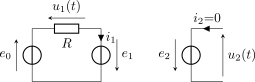
\includegraphics[scale=1]{indmutcorr}
		      \caption{Schéma électrique équivalent au dispositif de mesure
			      d'inductance mutuelle.}
		      \label{fig:indmutcorr}
	      \end{figure}
	      Pour obtenir un lien entre la tension de droite et la tension $u_1(t)$ à
	      gauche, il est donc nécessaire d'utiliser la loi de \textsc{Faraday} sur
	      au moins l'un des deux circuits. Par exemple, directement sur le circuit
	      de $L_2$ et en prenant bien $e_2 = -u_2$, on trouve
	      \[
		      e_2 = -L_2 \dv{i_2}{t} - M \dv{i_1}{t}
	      \]
	      et avec la RCT sur la résistance, $u_1 = R i_1$, on a
	      \[
		      u_2 = M \dv{i_1}{t}
		      \qso
		      \boxed{\frac{M}{R} \dv{u_1}{t}}
	      \]
	\item À partir de la relation précédente et connaissant les amplitudes des
	      signaux électriques, on voudrait calculer $M$. Étant donné que l'entrée
	      est sinusoïdale, en RSF on s'attend à ce que la sortie soit sinusoïdale
	      également, et on peut passer en complexes pour obtenir une relation sur
	      les amplitudes complexes~:
	      \[
		      \ul{U_2} = \jw \frac{M}{R} \ul{U_1}
	      \]
	      et avec $U_{1,2} = \abs{\ul{U_{1,2}}}$, on obtient
	      \begin{gather*}
		      U_2 = \w \frac{M}{R} U_1
		      \Lra
		      \boxed{M = \frac{RU_2}{2\pi fU_1}}
		      \qav
		      \left\{
		      \begin{array}{rcl}
			      R   & = & \SI{100}{\Omega}
			      \\
			      U_2 & = & \SI{0.5}{V}
			      \\
			      U_1 & = & \SI{3.00}{V}
			      \\
			      f   & = & \SI{2.0}{kHz}
		      \end{array}
		      \right.
		      \\
		      \mathrm{A.N.~:}\enskip
		      \ul{
			      M = \SI{1.3}{mH}
		      }
	      \end{gather*}
	\item
	      \begin{enumerate}
		      \item Lorsque la bobine 2 est tournée de $\ang{180}$, elle retrouve
		            exactement la configuration géométrique de départ, excepté le
		            sens de branchement des fils, qui est inversé. On mesure alors
		            $u_2' = -u_2$, et le même calcul que précédemment montre que
		            \textbf{la valeur absolue de $M$ n'a pas changé}. On a en effet
		            les mêmes lignes de champ et la même surface totale, il n'y a
		            que son orientation qui varie. En toute rigueur, on aura $M' =
			            -M$.
		      \item Lorsque la bobine est tournée de $\ang{90}$, beaucoup moins de
		            lignes de champ issues de la bobine 1 ne traversent la bobine 2.
		            Le flux croisé $\F_{1 \ra 2}$ est donc nettement diminué alors
		            que $i_1$ est fixée~: c'est forcément que \textbf{$M$ est plus
			            faible}.
		      \item Au contraire, si la bobine 2 est placée sur le même axe que la
		            bobine 1, et à une distance comparable à la première situation,
		            alors davantage de lignes de champs de 1 traversent 2~: $\F_{1
				            \ra 2}$ augmente à $i_1$ fixé, donc \textbf{$M$ est plus
			            grande}.
	      \end{enumerate}
\end{enumerate}

\section{Solénoïdes imbriqués}
\label{sec:solimbcorr}
\begin{enumerate}
	\item Il faut savoir traduire la phrase classique de l'énoncé~: «~$\ell$ est
	      très supérieure aux rayons~». Mathématiquement, on a donc $\ell \gg r_1$
	      et $r_2$. Physiquement, cela permet d'approximer les solénoïdes comme
	      étant «~infinis~», donc \textbf{sans effet de bord} où les lignes de
	      champ ne sont plus parallèles et commencent à boucler. Ainsi, on pourra
	      utiliser l'expression du champ magnétique créé par un solénoïde en son
	      sein sans réserve quant aux bords.
	      \bigbreak
	      En notant $i_1$ et $i_2$ les courants (possiblement nuls) circulant dans
	      les bobines, et en tenant compte de l'orientation des spires, ce champ
	      dans chacune des bobines est
	      \[
		      \vv{B_{1,2}} = \mu_0 \frac{N}{\ell} i_{1,2} \ez
	      \]
	      \paragraph*{Inductance propre $L_1$}
	      \begin{itemize}
		      \item Flux créé par S$_1$ dans \textbf{une spire} $s_1$ d'elle-même~:
		            \[
			            \F_{\Sr_1 \ra s_1}
			            = \iint _{\Mr \in s_1} \vv{B_1}(\Mr) \cdot \dd{S}\ez
			            = \vv{B_1}\cdot \vv{S}
			            = \pi r_1{}^{2} \mu_0 \frac{N}{\ell}i_1
		            \]
		      \item Flux \textbf{propre} créé par S$_1$ dans \textbf{toutes ses
			            spires}~:
		            \[
			            \F_{p,1} = \F_{\Sr_1 \ra \Sr_1} = N \times \F_{\Sr_1 \ra s_1}
			            \qdc
			            \F_{p,1} = \pi r_1{}^{2} \mu_0 \frac{N^2}{\ell}i_1
		            \]
		      \item Inductance propre~: par \textbf{définition}, $\F_{p,1} =
			            L_1i_1$, soit
		            \[
			            \boxed{L_1 = \pi r_1{}^{2} \mu_0 \frac{N^2}{\ell}}
		            \]
	      \end{itemize}
	      \paragraph*{Inductance propre $L_2$}
	      Par la même démarche, et ce même si $i_2 = 0$, on trouve
	      \[
		      \boxed{L_2 = \pi r_2{}^{2}\mu_0 \frac{N^2}{\ell}}
	      \]
	      et elle ne dépendent bien que du circuit, et pas de l'intensité.
	      \paragraph*{Inductance mutuelle}
	      Comme le champ créé par S$_2$ est uniforme à l'intérieur de $S_1$ (la
	      réciproque n'est pas vraie~!), il suffit de calculer ce flux croisé pour
	      obtenir $M$.
	      \begin{itemize}
		      \item Flux créé par S$_2$ au travers d'une spire $s_1$ de S$_1$~:
		            \[
			            \F_{\Sr_2 \ra s_1}
			            = \oiint_{\Mr \mathrlap{\in s_1}} \vv{B_2}(\Mr)\cdot \dd{S}\ez
			            = \pi r_1{}^{2} \mu_0 \frac{N}{\ell}i_2
		            \]
		      \item Flux \textbf{croisé} créé par S$_2$ dans \textbf{tout S$_1$}~:
		            \[
			            \F_{2\ra 1} = \F_{\Sr_2\ra\Sr_1} = N \F_{\Sr_2\ra s_1}
			            \qdc
			            \F_{2\ra 1} = \pi r_1{}^{2} \mu_0 \frac{N_2}{\ell}i_2
		            \]
		      \item Inductance mutuelle~: par \textbf{définition}, $\F_{2\ra 1} =
			            Mi_2$, soit
		            \[
			            \boxed{M = \pi r_1{}^{2} \mu_0 \frac{N^2}{\ell}}
		            \]
	      \end{itemize}
	\item Le circuit équivalent est tracé Figure~\ref{fig:solimbcorr}. Le circuit
	      1 contient une bobine et un générateur de \textbf{courant}, imposant le
	      courant $i_1$~; le circuit 2 ne contient qu'une bobine court-circuitée.
	      Il a couplage inductif entre les deux circuits, donc on prend en compte
	      les deux flux qui traversent chaque bobine pour utiliser la loi de
	      \textsc{Faraday}. En convention récepteur, on a pour la deuxième~:
	      \begin{figure}[htbp]
		      \centering
		      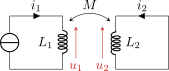
\includegraphics[scale=1]{solimbcorr}
		      \caption{Circuit électrique équivalent}
		      \label{fig:solimbcorr}
	      \end{figure}
	      \[
		      u_2 = +L_2 \dv{i_2}{t} + M \dv{i_1}{t}
	      \]
	      et il nous faut alors une relation électrique pour relier tension et
	      courant~: loi des mailles ou loi des nœuds. Ici, la loi des mailles sur
	      le circuit de droite donne simplement $u_2 = 0$, d'où
	      \begin{DispWithArrows*}
		      \dv{i_2}{t} &= - \frac{M}{L_2} \dv{i_1}{t}
		      \Arrow{par intégration} \\
		      \Ra
		      i_2 &= -\frac{M}{L_2}i_1 + \cte
	      \end{DispWithArrows*}
	      \textbf{sans oublier la constante}. Cependant, comme le solénoïde S$_2$
	      n'est pas relié à un générateur, il n'y a aucune raison pour qu'un
	      courant continu existe dans le circuit~; notamment, prendre $i_1 = 0
		      \forall t$ nous amène bien à remarquer que $\cte = 0$. Ainsi, en
	      remplaçant $i_1$ par son expression on obtient
	      \[
		      \boxed{i_2(t) = -\frac{M}{L_2}I\cos{\wt}}
		      \quad \text{d'amplitude} \quad
		      \boxed{I_2 = \frac{M}{L_2}I}
	      \]
	      On fera en effet bien attention à ne pas prendre le signe «~-~» dans
	      l'amplitude de $I_2$~: $I_2 = \abs{\max{I_2}}$.
	\item D'après le principe de superposition, en un point $\Mr$ se trouvant à
	      l'intérieur des deux solénoïdes on trouve
	      \[
		      \vv{B}(\Mr)
		      = \vv{B_1}(\Mr) + \vv{B_2}(\Mr)
		      = \mu_0 \frac{N}{l}(i_1+i_2) \ez
	      \]
	      et en factorisant par $i_1$ et en le remplaçant par son expression~:
	      \[
		      \boxed{
			      \vv{B}(\Mr) = \mu \frac{N}{\ell}
			      \left( 1 - \frac{M}{L} \right)I \cos(\wt)\ez
		      }
	      \]
\end{enumerate}

\section{Plaque de cuisson à induction}
\label{sec:plqindcorr}
\begin{enumerate}
	\item Un schéma de principe et un schéma électrique équivalent faisant
	      apparaître des générateurs induits sont représentés
	      Figure~\ref{fig:plqindcorr}. On peut raisonner indifféremment sur l'un
	      ou sur l'autre, à condition de se méfier de la loi de comportement de la
	      bobine si on choisit le schéma de gauche, et de ne pas oublier
	      l'auto-induction si on choisit le schéma de droite.
	      \begin{figure}[htbp]
		      \centering
		      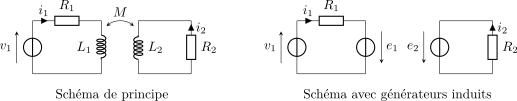
\includegraphics[scale=1]{plqindcorr}
		      \caption{Schémas équivalents à une plaque à induction.}
		      \label{fig:plqindcorr}
	      \end{figure}
	      Pour obtenir les tensions dans les bobines, il faut prendre en compte
	      l'auto-induction ainsi que l'induction mutuelle. Par définition,
	      \[
		      \F_{1} = \F_{p,1} + \F_{2 \ra 1}
		      \qet
		      \F_{p,1} = L_1 i_1
		      \quad;\quad
		      \F_{2 \ra 1} = M i_2
		      \qqdc
		      e_1 = -\dv{\F_1}{t} = -L_1 \dv{i_1}{t} - M \dv{i_2}{t}
	      \]
	      mais également
	      \[
		      \F_{2} = \F_{p,2} + \F_{1 \ra 2}
		      \qet
		      \F_{p,2} = L_2 i_2
		      \quad;\quad
		      \F_{1 \ra 2} = M i_1
		      \qqdc
		      e_2 = -\dv{\F_2}{t} = -L_2 \dv{i_2}{t} - M \dv{i_1}{t}
	      \]
	      Pour les relier entre elles, on doit trouver d'autres équations
	      électriques~; ici avec la loi des mailles~:
	      \[
		      v_1 + e_1 = R_1i_1
		      \qet
		      e_2 = R_2i_2
	      \]
	      d'où finalement
	      \begin{empheq}[left=\empheqlbrace]{align}
		      \label{eq:plq1}
		      v_1 & = R_1i_1 + L_1 \dv{i_1}{t} + M \dv{i_2}{t}
		      \\
		      \label{eq:plq2}
		      0 & = R_2i_2 + L_2 \dv{i_2}{t} + M \dv{i_1}{t}
	      \end{empheq}
	\item Parmi ces deux équations, la \ref{eq:plq2} est plus simple pour
	      obtenir la fraction demandée puisque la première fait intervenir $v_1$.
	      En la passant en complexes~:
	      \begin{align}
		      0              & = R_2 \ul{I_2} + \jw L_2 \ul{I_2} + \jw M \ul{I_1}
		      \notag
		      \\\Lra
		      \label{eq:plq3}
		      \Aboxed{\ul{H} & = - \frac{\jw M}{R_2+\jw L_2}}
	      \end{align}
	\item Avec l'équation \ref{eq:plq1}, on obtient
	      \begin{align}
		      \ul{V_1}                             & =
		      (R_1 + \jw L_1)\ul{I_1} + \jw M \ul{I_2}
		      \notag
		      \\\Lra
		      \ul{Z_e} = \frac{\ul{V_1}}{\ul{I_1}} & =
		      R_1 + \jw L_1 + \jw M \ul{H}
		      \notag
		      \\\Lra
		      \label{eq:plq4}
		      \Aboxed{\ul{Z_e}                     & =
			      R_1 + \jw L_1 + \frac{(M\w)^2}{R_2 + \jw L_2}}
	      \end{align}
	\item $\w \gg R_2/L_2$ et $\w \gg R_1/L_1$ nous guide vers l'idée de
	      prendre $\w \ra +\infty$. On va faire apparaître ça en factorisant par
	      $L_2$ en haut et en bas de l'équation \ref{eq:plq3}~:
	      \[
		      \ul{H} = - \cancel{\frac{L_2}{L_2}} \frac{\jw M/L_2}{R_2/L_2 + \jw}
		      \Lra
		      \ul{H} \underset{\w \to \infty}{\sim} \frac{\jw M/L_2}{\jw +
			      \underbracket{\dcancel{R_2/L_2}}_{\ll \w}}
		      \Lra
		      \boxed{\ul{H} \underset{\w \to \infty}{\sim} - \frac{M}{L_2}}
	      \]
	      qu'on réinjecte ensuite dans l'équation \ref{eq:plq4}~:
	      \[
		      \boxed{\ul{Z_e} = \jw L_1 \left( 1 - \frac{M^2}{L_1L_2} \right)}
	      \]
	      Ainsi,
	      \[
		      \ul{\abs{\frac{\ul{I_2}}{I_1}} = \num{8.3}}
		      \qet
		      \ul{\abs{\ul{Z_e}} = \SI{2.1}{\Omega}}
		      \qav
		      \left\{
		      \begin{array}{rcl}
			      M   & = & \SI{2}{\micro H}
			      \\
			      L_1 & = & \SI{30}{\micro H}
			      \\
			      L_2 & = & \SI{0.24}{\micro H}
			      \\
			      \w  & = & \SI{7.0e4}{rad.s^{-1}}
		      \end{array}
		      \right.
	      \]
	      \begin{rrema}{Remarque}
		      On remarque que la qualité du couplage inductif apparaît dans l'expression
		      de $\ul{Z_e}$~: si le couplage est parfait, alors $M = \sqrt{L_1L_2}$,
		      donc l'impédance d'entrée du système est nulle, signe d'une transmission
		      parfaite de l'énergie électromagnétique. On retrouve exactement le même
		      résultat à propos du transformateur.
		      \bigbreak
		      Remarque aussi que la différence de nombre de spires dans l'inducteur et
		      l'induit permet au courant à l'induit d'être nettement supérieur au
		      courant à l'inducteur, et donc de fournir davantage d'effet \textsc{Joule}
		      dans le fond de la casserole que dans la plaque.
	      \end{rrema}
	\item Qualitativement, si l'on éloigne la casserole le couplage sera moins
	      bon ($M$ diminue). Ainsi, l'\textbf{impédance d'entrée
		      augmente}\footnote{Plus précisément, comme la casserole est éloignée de
		      l'inducteur qui est source de champ magnétique, le flux vu par
		      l'induit diminue, combien même le courant dans l'induction serait
		      imposé, ce qui indique que $M$ diminue.}. Si l'impédance d'entrée
	      augmente alors que $v_1$ ne change pas, étant donné que $\ul{Z_e} =
		      \ul{V_1}/\ul{I}$ on en déduit que \textbf{l'inducteur appelle moins de
		      courant}.
\end{enumerate}

\section{Peut-on négliger l'auto-induction~?}
\label{sec:neglautoindcorr}
\begin{enumerate}
	\item Compte-tenu du sens de $i$ sur le schéma, levecteur normal orienté est
	      le vecteur $+\vv{n}$. Ainsi,
	      \[
		      \F_{\ext} = S \vv{B}_{\ext}\cdot \vv{n} = S B_0 \cos(\wt)
	      \]
	      Sur le schéma électrique Figure~\ref{fig:neglautoindcorr}, la f.é.m.\
	      induite $e_{\ext}$ est orientée \ul{dans le même sens} que l'intensité,
	      et vaut
	      \[
		      e_{\ext} = -\dv{\F_{\ext}}{t} = + SB_0\w \sin(\wt)
	      \]
	      d'où on déduit l'intensité induite par le champ extérieur $i_{\ext} =
		      e_{\ext}/R$ de la loi d'\textsc{Ohm},
	      \[
		      \boxed{i_{\ext} = \frac{SB_0\w}{R}\sin(\wt)}
	      \]
	      \begin{figure}[htbp]
		      \centering
		      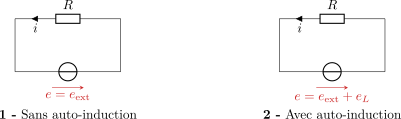
\includegraphics[scale=1]{autoindneglcorr}
		      \caption{Schémas électriques équivalents.}
		      \label{fig:neglautoindcorr}
	      \end{figure}
	\item En tenant compte de l'auto-induction,
	      \[
		      \F = \F_{\ext} + Li
		      \qdc
		      \F = SB_0 \cos(\wt) + Li
	      \]
	      \begin{tror}{Attention}
		      Il n'est pas possible de remplacer $i$ par l'expression obtenue à la
		      question précédente~: cette expression n'est valable que lorsque seul
		      le champ extérieur est pris en compte, or nous nous intéressons
		      désormais en plus à l'auto-induction.
	      \end{tror}
	      Le schéma électrique équivalent est représente
	      Figure~\ref{fig:neglautoindcorr}. La f.é.m.\ induite tient compte des
	      deux contributions au flux, et vaut
	      \[
		      e = -\dv{\F}{t} = SB_0 \sin(\wt) - L \dv{i}{t}
	      \]
	      D'après la loi des mailles et la loi d'\textsc{Ohm}, on a $e = Ri$, d'où
	      \begin{equation}
		      \label{eq:autoindnegl1}
		      \boxed{L \dv{i}{t} + Ri = SB_0\w \sin(\wt)}
	      \end{equation}
	\item À partir des raisonnements précédents, on identifie
	      \[
		      e_{\ext} = - \dv{\F_{\ext}}{t}
		      \qdc
		      \ul{E}_{\ext} = \jw SB_0
	      \]
	      et de même
	      \[
		      e_{L} = -L\dv{i}{t}
		      \qdc
		      \ul{E}_{L} = -\jw L \ul{I}
	      \]
	      d'où on trouve
	      \[
		      \ul{H} = \ul{E}_{L}/\ul{E}_{\ext} =
		      \frac{-\jw L \ul{I}}{\jw S B_0} = \frac{L}{SB_0} \ul{I}
	      \]
	      Or, d'après l'équation différentielle \eqref{eq:autoindnegl1},
	      \[
		      \jw L \ul{I} + R \ul{I} = \jw SB_0
		      \qso
		      \ul{I} = \frac{\jw SB_0}{R + \jw L}
	      \]
	      L'expression finale est donc
	      \[
		      \ul{H} = \frac{L}{SB_0} \frac{\jw SB_0}{R + \jw L}
		      \qdc
		      \boxed{\abs{\ul{H}} = \frac{L\w}{\sqrt{R^2 + L^2w^2}}
			      = \frac{1}{\sqrt{1+\frac{R^2}{L^2w^2}}}}
	      \]
	      La force électromotrice auto-induite est négligeable devant l'induite
	      dès lors que $\abs{\ul{H}} \ll 1$, c'est-à-dire lorsque $R/L\w \gg 1$,
	      soit
	      \[
		      \boxed{\w \ll \frac{R}{L}}
	      \]
	      Pour reprendre des termes plus familiers en électrocinétique, on vient
	      d’établir que la f.é.m.\ auto-induite de la bobine était négligeable en
	      régime très basse fréquence… là même où l'on affirmait plus tôt dans
	      l'année qu'elle était équivalente à un fil, c'est-à-dire que son
	      comportement «~bobine~» n’apparaissait pas. Comme le comportement
	      «~bobine~» est justement de l'auto-induction… la boucle est bouclée~!
	\item Pour $L = \SI{100}{mH}$ et $R = \SI{1}{k\Omega}$, l'auto-induction est
	      négligeable dans la limite
	      \[
		      \boxed{
			      \w \ll \SI{1e4}{rad.s^{-1}}
			      \qso
			      f \ll \SI{1.6}{kHz}}
	      \]
	\item Considérons par exemple $d \approx \SI{1}{mm}$ et $D \approx \SI{1}{m}$.
	      On trouve alors $L \approx \SI{4e-6}{H}$, ce qui donne comme condition
	      \[
		      \w \ll \SI{2e9}{rad.s^{-1}}
		      \qso
		      f \ll \SI{3e8}{Hz}
	      \]
	      Pour toutes les fréquences usuelles en électronique, limitées au plus à
	      \SI{1e7}{Hz}, \textbf{négliger l'auto-induction du circuit est donc
		      légitime}.
\end{enumerate}

\section{Principe de fonctionnement d'un générateur synchrone \hfill \small oral
  CCP}
\label{sec:motsynchcorr}

\begin{enumerate}
	\item Comme la distance entre la spire et l'aimant est bien plus grande que le
	      rayon de la spire, on peut considérer le champ magnétique généra par
	      l'aimant uniforme, et vaut
	      \[
		      \vv{B}_{a}(\tt) = \frac{\mu_0 m_0}{4\pi x^3}
		      (2\cos{\theta}\ur + \sin{\theta}\ut)
	      \]
	      en étant très vigilant-e à la définition de l'angle $\tt$ servant à
	      repérer la position de la spire, voir Figure~\ref{fig:motsynchcorr}.
	      \begin{figure}[htbp]
		      \centering
		      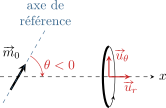
\includegraphics[scale=1]{motsynchcorr}
		      \caption{Orientation relative de la spire par rapport à l'aimant.}
		      \label{fig:motsynchcorr}
	      \end{figure}
	      Compte-tenu de l'orientation de la spire, spécifiée sur le schéma, le
	      flux du champ magnétique au travers de la spire vaut
	      \[
		      \F = S \vv{B}_a \cdot \ur = \pi a^2 \times \frac{\mu_0 m_0}{4\pi x^3}
		      \times 2\cos{\theta} = \frac{\mu_0 m_0 a^2}{2x^3}\cos{\theta}
	      \]
	      et on en déduit la force électromotrice induit dans la spire
	      \[
		      e = -\dv{\f}{t} = -\frac{\mu_0 m_0 a^2}{2x^3}
		      \left( - \tp \sin{\theta} \right)
	      \]
	      Si l'aimant tourne à vitesse angulaire $\w$ constante autour de l'axe
	      $z$, alors compte-tenu du schéma on a $\tt = -\wt$ (en supposant $\tt =
		      0$ à $t=0$), donc $\tp = -\w$, et ainsi
	      \[
		      e = + \frac{\mu_0 m_0a^2}{2x^3} \w \sin{\wt}
	      \]
	      \begin{tror}{Attention}
		      Faites très attention aux multiples signes et compensations de signe~!
		      Vérifiez également qualitativement le signe final~: pour $t=0$,
		      l'aimant est dans l'axe de la spire, donc à $t \gtrsim 0$ il s'en
		      éloigne~; donc le flux au travers de la spire diminue, donc d'après la
		      loi de \textsc{Faraday} $e > 0$. C'est bien ce qu'on vient de
		      trouver~!
	      \end{tror}
	      Le courant induite se détermine alors directement à partir de la loi
	      d'\textsc{Ohm}, $i = e/R$, d'où
	      \[
		      \boxed{i = \frac{\mu_0 m_0 a^2 \w}{2x^3R} \sin(\wt)}
	      \]
	      La spire étant simplement résistive, elle ne peut stocker d'énergie, et
	      toute la puissance qu'elle reçoit est dissipée par effet \textsc{Joule}.
	      Ainsi, la puissance électrique reçue par la spire $\Pc_e = Ri^2$ vaut
	      \[
		      \boxed{\Pc_e = \frac{1}{R} \left( \frac{\mu_0 m_0a^2\w}{2x^3} \right)^{2}
			      \sin^2(\wt)}
	      \]
	\item Le champ créé par l'aimant n'exerce pas de couple sur l'aimant lui-même.
	      On en déduit que le champ à l'origine de ce couple est donc dans le
	      champ magnétique induit par la spire. L'énoncé donne le champ créé par
	      un moment magnétique~: il faut donc calculer le moment magnétique de la
	      spire pour en déduire le champ qu'elle créé, en étant particulièrement
	      vigilant-e au repérage. Compte-tenu de l'orientation du courant sur la
	      Figure~\ref{fig:motsynchcorr}, le moment magnétique de la spire vaut
	      \[
		      \vv{m}_{\rm sp} = i\pi a^2 \ux = \frac{\pi \mu_0 m_0 a^4\w}{2x^3R}
		      \sin{\wt} \ux
	      \]
	      En coordonnées polaires d'axe $\ux$ et d'origine le centre \textbf{de la
		      spire} (et donc pas O~!), l'aimant a pour coordonnées $r =x$ et $\tt =
		      \pi$, si bien que $\ur = -\ux$ et $\ut = -\uy$. On en déduit que le
	      champ magnétique créé en O au niveau de l'aimant par la spire vaut
	      \begin{DispWithArrows*}[]
		      \vv{B}_{\rm sp}(\Or) &=
		      \frac{\mu_0 m_{\rm sp}}{4\pi x^3}
		      \left[ 2 \underbracket{\cos(\pi)}_{=-1}(-\ux)
			      + \underbracket{\sin(\pi)}_{=0}(-\uy) \right]
		      \Arrow{$\DS m_{\rm sp} = \frac{\pi \mu_0 m_0 a^4\w}{2x^3R} \sin{\wt}$}
		      \\\Lra
		      \vv{B}_{\rm sp}(\Or) &=
		      \frac{\mu_0}{4\pi x^3} \times \frac{\pi \mu_0 m_0 a^4\w}{2x^3R}
		      \sin{\wt} \times 2 \ux
		      \\\Lra
		      \vv{B}_{\rm sp}(\Or) &=
		      \frac{\mu_0{}^{2}m_0 a^4\w}{4x^6} \sin{\wt}\ux
	      \end{DispWithArrows*}
	      \begin{tror}{Attention}
		      Ici aussi, pensez à \textbf{vérifier qualitativement les signes}~:
		      d'après la question précédente, $i>0$ pour $t \gtrsim 0$, donc avec la
		      règle de la main droite on a $\vv{B}_{\rm sp}$ porté par $+\ux$.
		      \smallbreak
		      Compte-tenu du fait que les calculs ne sont pas très sympathiques, ces
		      vérifications qualitatives font partie intégrante des compétences
		      testées à l'oral des concours.
	      \end{tror}
	      Finalement, le couple magnétique exercé par la spire sur l'aimant vaut
	      \[
		      \vv{\Gamma} = \vv{m_0} \wedge \vv{B}_{\rm sp} (\Or)
	      \]
	      Le plus sûr pour calculer le produit vectoriel est de décomposer les
	      coordonnées de $\vv{m_0}$ sur la base $\ux, \uy$. Comme l'aimant tourne
	      à vitesse angulaire $\w$ supposée positive autour de $\uz$, alors
	      \begin{DispWithArrows*}[]
		      \vv{\Gamma} &= m_0 [\cos(\wt)\ux + \sin(\wt)\uy]
		      \wedge \frac{\mu_0{}^{2}m_0 a^4 \w}{4x^6R}\sin(\wt) \ux
		      \Arrow{$\ux \wedge \ux = \vv{0}$\\$\uy \wedge \ux = -\uz$}
		      \\\Lra
		      \Aboxed{\vv{\Gamma} &= -\frac{\mu_0{}^{2}m_0{}^{2}a^4\w}{4x^6R}
		      \sin^2(\wt)\uz}
	      \end{DispWithArrows*}
	      \begin{tror}{Vérification}
		      Ici encore, le couple est porté par $-\uz$, c'est-à-dire qu'il
		      \textbf{résiste} au mouvement de l'aimant. D'après la loi de
		      \textsc{Lenz}, c'est complètement normal, puisque ce couple est
		      d'origine inductive, et que la cause de ce phénomène d'induction est
		      le mouvement de l'aimant.
	      \end{tror}
	\item Pour maintenir la vitesse de rotation de l'aimant constante, le système
	      mécanique doit fournir à l'aimant une puissance, sous forme d'un couple,
	      exactement opposée à la puissance dissipée par $\vv{\Gamma}$. La
	      puissance mécanique à fournir vaut donc $\Pc_m = -\Gamma\w$, d'où
	      \[
		      \boxed{\Pc_m = \frac{\mu_0{}^{2}m_0{}^{2}a^4\w^2}{4x^6R}\sin^2(\wt)}
	      \]
	      On remarque qu'on a $\Pc_m = \Pc_e$, c'est-à-dire que \textbf{toute la
		      puissance mécanique fournie à l'aimant est transmise à la spire sous
		      forme de puissance électrique~: on a bien modélisé un générateur
		      électrique simplifié.}
\end{enumerate}

\end{document}
